% Options for packages loaded elsewhere
\PassOptionsToPackage{unicode}{hyperref}
\PassOptionsToPackage{hyphens}{url}
\PassOptionsToPackage{dvipsnames,svgnames,x11names}{xcolor}
%
\documentclass[
  8pt,
  ignorenonframetext,
]{beamer}
\title{Programmation sous R\\
Chapitre 2: Graphiques - Statistiques}
\author{Mohamed Essaied Hamrita\\
\href{mailto:mhamrita@gmail.com}{\nolinkurl{mhamrita@gmail.com}}\\
\href{https:github.com/Hamrita}{github.com/Hamrita}}
\date{2023-2024}
\institute{Université de Sousse - Tunisie}

\usepackage{pgfpages}
\setbeamertemplate{caption}[numbered]
\setbeamertemplate{caption label separator}{: }
\setbeamercolor{caption name}{fg=normal text.fg}
\beamertemplatenavigationsymbolsempty
% Prevent slide breaks in the middle of a paragraph
\widowpenalties 1 10000
\raggedbottom
\setbeamertemplate{part page}{
  \centering
  \begin{beamercolorbox}[sep=16pt,center]{part title}
    \usebeamerfont{part title}\insertpart\par
  \end{beamercolorbox}
}
\setbeamertemplate{section page}{
  \centering
  \begin{beamercolorbox}[sep=12pt,center]{part title}
    \usebeamerfont{section title}\insertsection\par
  \end{beamercolorbox}
}
\setbeamertemplate{subsection page}{
  \centering
  \begin{beamercolorbox}[sep=8pt,center]{part title}
    \usebeamerfont{subsection title}\insertsubsection\par
  \end{beamercolorbox}
}
\AtBeginPart{
  \frame{\partpage}
}
\AtBeginSection{
  \ifbibliography
  \else
    \frame{\sectionpage}
  \fi
}
\AtBeginSubsection{
  \frame{\subsectionpage}
}
\usepackage{amsmath,amssymb}
\usepackage{lmodern}
\usepackage{iftex}
\ifPDFTeX
  \usepackage[T1]{fontenc}
  \usepackage[utf8]{inputenc}
  \usepackage{textcomp} % provide euro and other symbols
\else % if luatex or xetex
  \usepackage{unicode-math}
  \defaultfontfeatures{Scale=MatchLowercase}
  \defaultfontfeatures[\rmfamily]{Ligatures=TeX,Scale=1}
\fi
\usetheme[]{Frankfurt}
\usecolortheme{dolphin}
\usefonttheme{professionalfonts}
% Use upquote if available, for straight quotes in verbatim environments
\IfFileExists{upquote.sty}{\usepackage{upquote}}{}
\IfFileExists{microtype.sty}{% use microtype if available
  \usepackage[]{microtype}
  \UseMicrotypeSet[protrusion]{basicmath} % disable protrusion for tt fonts
}{}
\makeatletter
\@ifundefined{KOMAClassName}{% if non-KOMA class
  \IfFileExists{parskip.sty}{%
    \usepackage{parskip}
  }{% else
    \setlength{\parindent}{0pt}
    \setlength{\parskip}{6pt plus 2pt minus 1pt}}
}{% if KOMA class
  \KOMAoptions{parskip=half}}
\makeatother
\usepackage{xcolor}
\IfFileExists{xurl.sty}{\usepackage{xurl}}{} % add URL line breaks if available
\IfFileExists{bookmark.sty}{\usepackage{bookmark}}{\usepackage{hyperref}}
\hypersetup{
  colorlinks=true,
  linkcolor={Maroon},
  filecolor={Maroon},
  citecolor={Blue},
  urlcolor={blue},
  pdfcreator={LaTeX via pandoc}}
\urlstyle{same} % disable monospaced font for URLs
\newif\ifbibliography
\usepackage{color}
\usepackage{fancyvrb}
\newcommand{\VerbBar}{|}
\newcommand{\VERB}{\Verb[commandchars=\\\{\}]}
\DefineVerbatimEnvironment{Highlighting}{Verbatim}{commandchars=\\\{\}}
% Add ',fontsize=\small' for more characters per line
\usepackage{framed}
\definecolor{shadecolor}{RGB}{248,248,248}
\newenvironment{Shaded}{\begin{snugshade}}{\end{snugshade}}
\newcommand{\AlertTok}[1]{\textcolor[rgb]{0.94,0.16,0.16}{#1}}
\newcommand{\AnnotationTok}[1]{\textcolor[rgb]{0.56,0.35,0.01}{\textbf{\textit{#1}}}}
\newcommand{\AttributeTok}[1]{\textcolor[rgb]{0.77,0.63,0.00}{#1}}
\newcommand{\BaseNTok}[1]{\textcolor[rgb]{0.00,0.00,0.81}{#1}}
\newcommand{\BuiltInTok}[1]{#1}
\newcommand{\CharTok}[1]{\textcolor[rgb]{0.31,0.60,0.02}{#1}}
\newcommand{\CommentTok}[1]{\textcolor[rgb]{0.56,0.35,0.01}{\textit{#1}}}
\newcommand{\CommentVarTok}[1]{\textcolor[rgb]{0.56,0.35,0.01}{\textbf{\textit{#1}}}}
\newcommand{\ConstantTok}[1]{\textcolor[rgb]{0.00,0.00,0.00}{#1}}
\newcommand{\ControlFlowTok}[1]{\textcolor[rgb]{0.13,0.29,0.53}{\textbf{#1}}}
\newcommand{\DataTypeTok}[1]{\textcolor[rgb]{0.13,0.29,0.53}{#1}}
\newcommand{\DecValTok}[1]{\textcolor[rgb]{0.00,0.00,0.81}{#1}}
\newcommand{\DocumentationTok}[1]{\textcolor[rgb]{0.56,0.35,0.01}{\textbf{\textit{#1}}}}
\newcommand{\ErrorTok}[1]{\textcolor[rgb]{0.64,0.00,0.00}{\textbf{#1}}}
\newcommand{\ExtensionTok}[1]{#1}
\newcommand{\FloatTok}[1]{\textcolor[rgb]{0.00,0.00,0.81}{#1}}
\newcommand{\FunctionTok}[1]{\textcolor[rgb]{0.00,0.00,0.00}{#1}}
\newcommand{\ImportTok}[1]{#1}
\newcommand{\InformationTok}[1]{\textcolor[rgb]{0.56,0.35,0.01}{\textbf{\textit{#1}}}}
\newcommand{\KeywordTok}[1]{\textcolor[rgb]{0.13,0.29,0.53}{\textbf{#1}}}
\newcommand{\NormalTok}[1]{#1}
\newcommand{\OperatorTok}[1]{\textcolor[rgb]{0.81,0.36,0.00}{\textbf{#1}}}
\newcommand{\OtherTok}[1]{\textcolor[rgb]{0.56,0.35,0.01}{#1}}
\newcommand{\PreprocessorTok}[1]{\textcolor[rgb]{0.56,0.35,0.01}{\textit{#1}}}
\newcommand{\RegionMarkerTok}[1]{#1}
\newcommand{\SpecialCharTok}[1]{\textcolor[rgb]{0.00,0.00,0.00}{#1}}
\newcommand{\SpecialStringTok}[1]{\textcolor[rgb]{0.31,0.60,0.02}{#1}}
\newcommand{\StringTok}[1]{\textcolor[rgb]{0.31,0.60,0.02}{#1}}
\newcommand{\VariableTok}[1]{\textcolor[rgb]{0.00,0.00,0.00}{#1}}
\newcommand{\VerbatimStringTok}[1]{\textcolor[rgb]{0.31,0.60,0.02}{#1}}
\newcommand{\WarningTok}[1]{\textcolor[rgb]{0.56,0.35,0.01}{\textbf{\textit{#1}}}}
\usepackage{longtable,booktabs,array}
\usepackage{calc} % for calculating minipage widths
\usepackage{caption}
% Make caption package work with longtable
\makeatletter
\def\fnum@table{\tablename~\thetable}
\makeatother
\usepackage{graphicx}
\makeatletter
\def\maxwidth{\ifdim\Gin@nat@width>\linewidth\linewidth\else\Gin@nat@width\fi}
\def\maxheight{\ifdim\Gin@nat@height>\textheight\textheight\else\Gin@nat@height\fi}
\makeatother
% Scale images if necessary, so that they will not overflow the page
% margins by default, and it is still possible to overwrite the defaults
% using explicit options in \includegraphics[width, height, ...]{}
\setkeys{Gin}{width=\maxwidth,height=\maxheight,keepaspectratio}
% Set default figure placement to htbp
\makeatletter
\def\fps@figure{htbp}
\makeatother
\setlength{\emergencystretch}{3em} % prevent overfull lines
\providecommand{\tightlist}{%
  \setlength{\itemsep}{0pt}\setlength{\parskip}{0pt}}
\setcounter{secnumdepth}{-\maxdimen} % remove section numbering
\setbeamertemplate{navigation symbols}{}
\setbeamertemplate{footline}[page number]
\ifLuaTeX
  \usepackage{selnolig}  % disable illegal ligatures
\fi

\begin{document}
\frame{\titlepage}

\begin{frame}[allowframebreaks]
  \tableofcontents[hideallsubsections]
\end{frame}
\hypertarget{graphiques}{%
\section{Graphiques}\label{graphiques}}

\begin{frame}[fragile]{Graphiques}
Cette section explique comment créer des types de graphique de base. La
commande la plus simple à utiliser pour représenter graphiquement un
ensemble de points est la commande \texttt{plot(x,y)}. La commande
\texttt{plot} a plusieurs arguments. Par défaut, cette commande trace
l'ensemble des points en points.

\begin{Shaded}
\begin{Highlighting}[]
\NormalTok{x}\OtherTok{=}\FunctionTok{c}\NormalTok{(}\SpecialCharTok{{-}}\DecValTok{2}\NormalTok{,}\DecValTok{1}\NormalTok{,}\DecValTok{5}\NormalTok{,}\SpecialCharTok{{-}}\DecValTok{4}\NormalTok{,}\DecValTok{0}\NormalTok{,}\DecValTok{3}\NormalTok{); }\FunctionTok{plot}\NormalTok{(x)}
\end{Highlighting}
\end{Shaded}

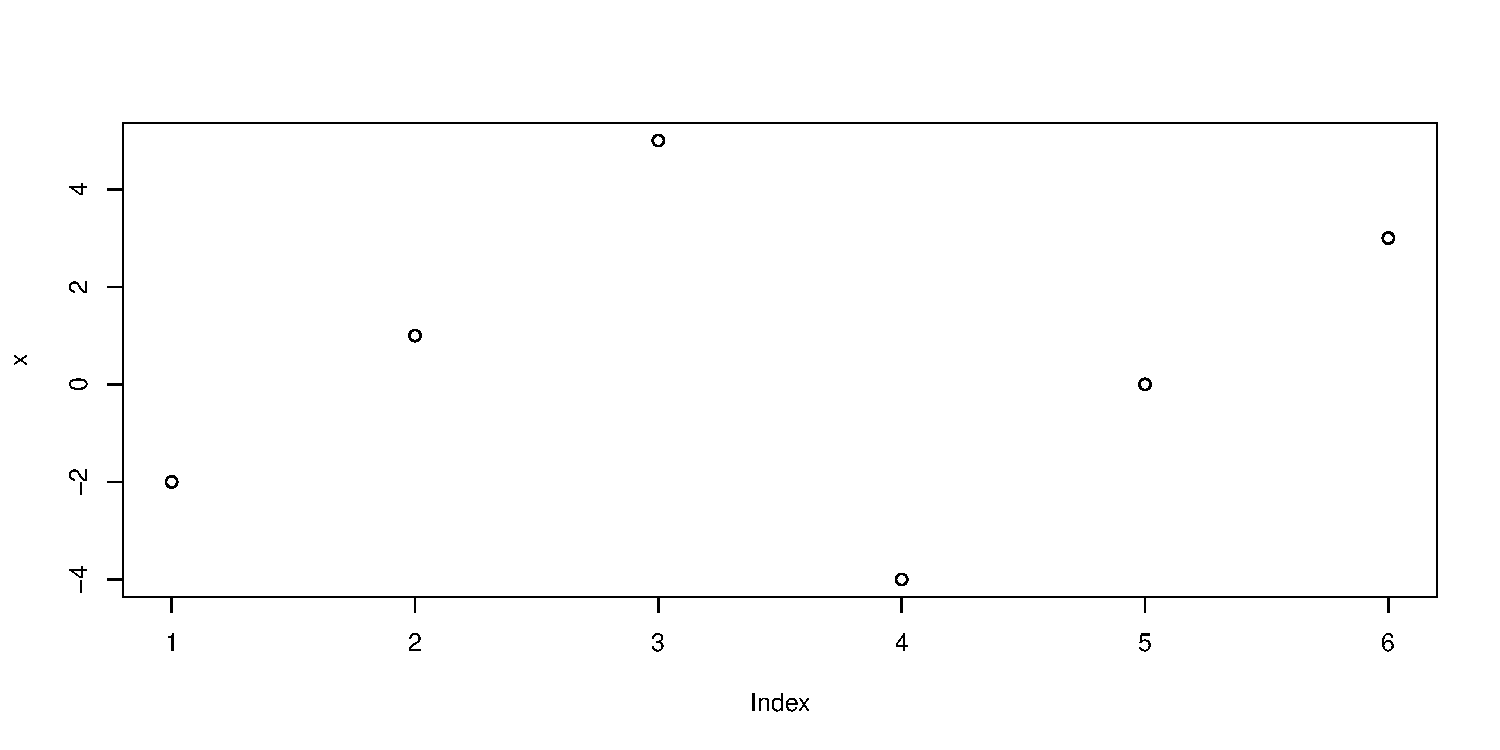
\includegraphics{Chap2_R_files/figure-beamer/unnamed-chunk-1-1.pdf}
\end{frame}

\begin{frame}[fragile]
Pour tracer une ligne, on doit ajouter l'argument \texttt{type="l"}.

\begin{Shaded}
\begin{Highlighting}[]
\FunctionTok{plot}\NormalTok{(x, }\AttributeTok{type=}\StringTok{"l"}\NormalTok{)}
\end{Highlighting}
\end{Shaded}

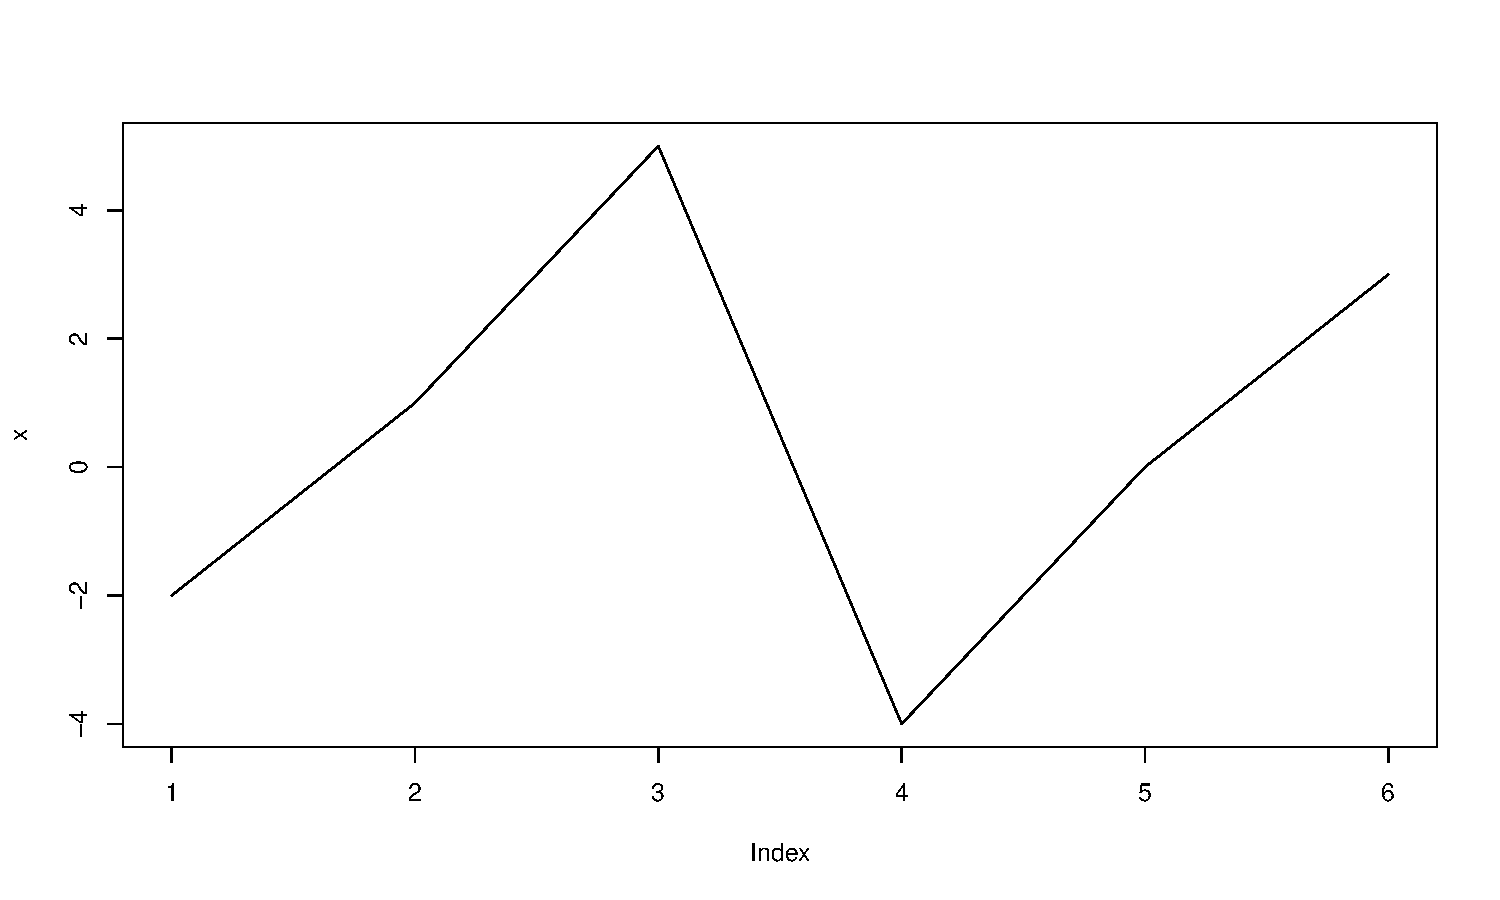
\includegraphics{Chap2_R_files/figure-beamer/unnamed-chunk-2-1.pdf}
\end{frame}

\begin{frame}[fragile]
Bien sûr, le logiciel \texttt{R} présente plusieurs arguments pour la
fonction plot, tels que le paramétrage des coleurs, largeur du trait de
la courbe, les étiquettes (labels) des axes, etc \ldots 

\begin{Shaded}
\begin{Highlighting}[]
\FunctionTok{plot}\NormalTok{(x,}\AttributeTok{type=}\StringTok{"l"}\NormalTok{, }\AttributeTok{col=}\StringTok{"red"}\NormalTok{,}\AttributeTok{lwd=}\DecValTok{2}\NormalTok{, }\AttributeTok{xlab=}\StringTok{"axes des abscisses"}\NormalTok{, }
\AttributeTok{ylab=}\StringTok{"axes des ordonnées"}\NormalTok{, }\AttributeTok{main=}\StringTok{"Mon premier graphique"}\NormalTok{, }
\AttributeTok{ylim=}\FunctionTok{c}\NormalTok{(}\SpecialCharTok{{-}}\DecValTok{6}\NormalTok{,}\DecValTok{6}\NormalTok{))}
\FunctionTok{points}\NormalTok{(x,}\AttributeTok{col=}\DecValTok{1}\SpecialCharTok{:}\DecValTok{6}\NormalTok{,}\AttributeTok{pch=}\DecValTok{1}\SpecialCharTok{:}\DecValTok{6}\NormalTok{,}\AttributeTok{lwd=}\DecValTok{3}\NormalTok{)}
\FunctionTok{legend}\NormalTok{(}\StringTok{"topleft"}\NormalTok{, }\StringTok{"Courbe"}\NormalTok{, }\AttributeTok{text.col=}\DecValTok{2}\NormalTok{, }\AttributeTok{lty=}\DecValTok{1}\NormalTok{)}
\end{Highlighting}
\end{Shaded}

\begin{center}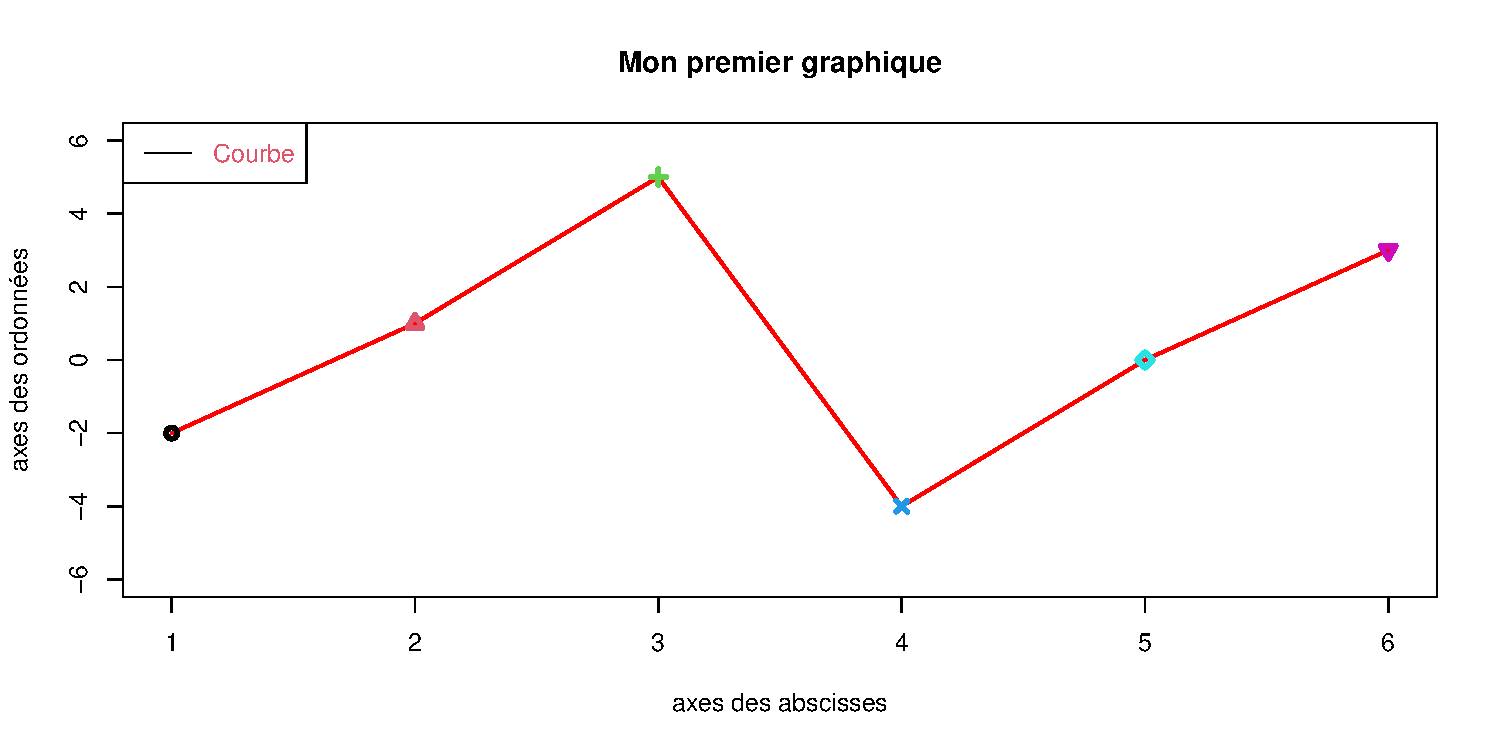
\includegraphics{Chap2_R_files/figure-beamer/unnamed-chunk-3-1} \end{center}
\end{frame}

\begin{frame}[fragile]
La représentation des courbes des fonctions peut être faite de deux
manières; soit par la fonction \texttt{plot}, soit par la fonction
\texttt{curve}.

\begin{Shaded}
\begin{Highlighting}[]
\NormalTok{xx}\OtherTok{=}\FunctionTok{seq}\NormalTok{(}\SpecialCharTok{{-}}\DecValTok{2}\SpecialCharTok{*}\NormalTok{pi, }\DecValTok{2}\SpecialCharTok{*}\NormalTok{pi, }\AttributeTok{len=}\DecValTok{100}\NormalTok{); yy}\OtherTok{=} \FunctionTok{sin}\NormalTok{(xx)}
\FunctionTok{plot}\NormalTok{(xx,yy,}\AttributeTok{type=}\StringTok{"l"}\NormalTok{,}\AttributeTok{xlab=}\StringTok{"x"}\NormalTok{, }\AttributeTok{ylab=}\FunctionTok{expression}\NormalTok{(}\FunctionTok{sin}\NormalTok{(x)), }
     \AttributeTok{col=}\DecValTok{2}\NormalTok{, }\AttributeTok{lwd=}\DecValTok{3}\NormalTok{)}
\FunctionTok{curve}\NormalTok{(cos, }\SpecialCharTok{{-}}\DecValTok{2}\SpecialCharTok{*}\NormalTok{pi, }\DecValTok{2}\SpecialCharTok{*}\NormalTok{pi, }\AttributeTok{col=}\DecValTok{4}\NormalTok{, }\AttributeTok{lwd=}\DecValTok{3}\NormalTok{, }\AttributeTok{lty=}\DecValTok{2}\NormalTok{, }\AttributeTok{add=}\NormalTok{T)}
\FunctionTok{legend}\NormalTok{(}\StringTok{"bottomleft"}\NormalTok{,}\FunctionTok{c}\NormalTok{(}\StringTok{"sin"}\NormalTok{, }\StringTok{"cos"}\NormalTok{), }\AttributeTok{lty=}\FunctionTok{c}\NormalTok{(}\DecValTok{1}\NormalTok{,}\DecValTok{2}\NormalTok{), }\AttributeTok{col=}\FunctionTok{c}\NormalTok{(}\DecValTok{2}\NormalTok{,}\DecValTok{4}\NormalTok{), }
       \AttributeTok{lwd=}\DecValTok{3}\NormalTok{,}\AttributeTok{bty=}\StringTok{"n"}\NormalTok{)}
\end{Highlighting}
\end{Shaded}

\begin{center}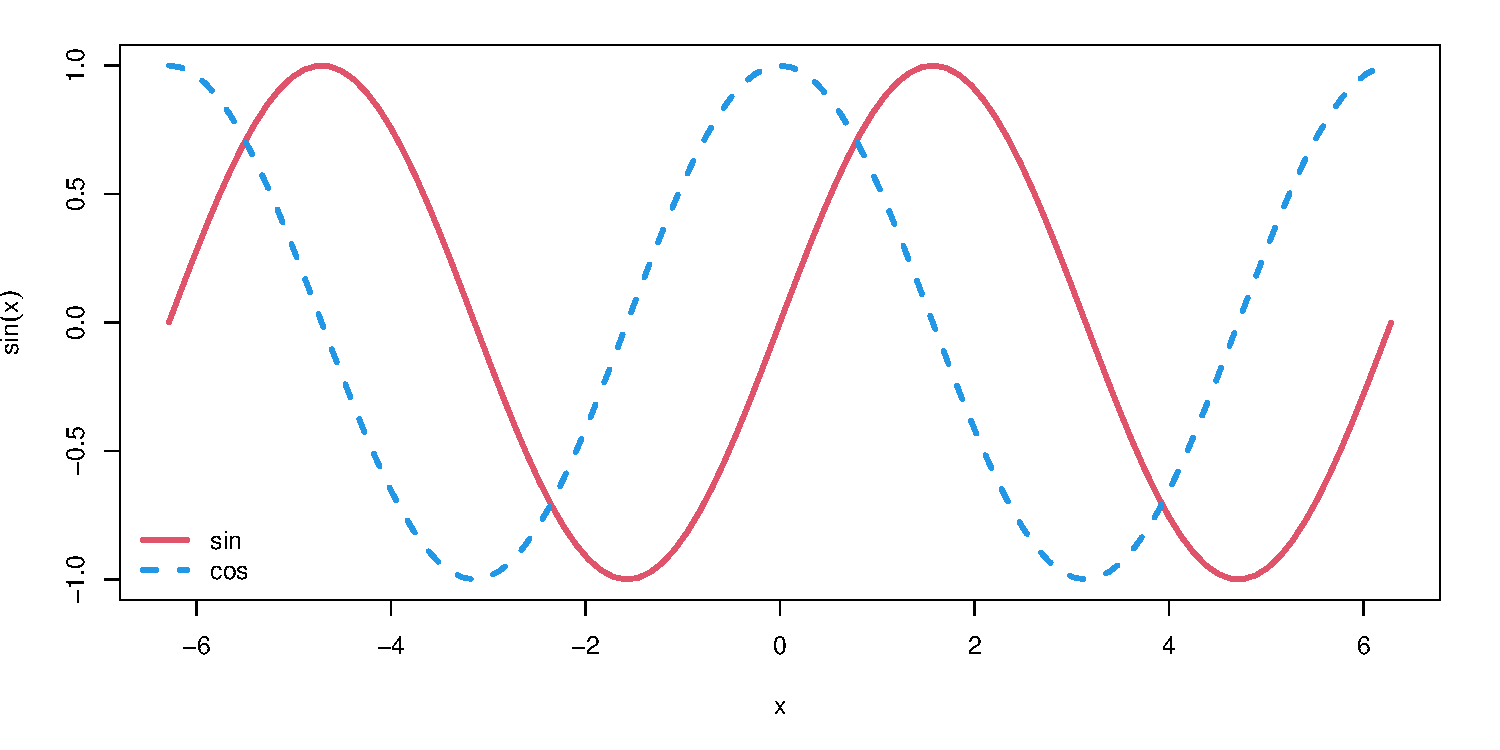
\includegraphics{Chap2_R_files/figure-beamer/unnamed-chunk-4-1} \end{center}
\end{frame}

\begin{frame}{Les symboles graphiques}
\protect\hypertarget{les-symboles-graphiques}{}
La figure ci-dessous montre les différents types de points:

\begin{center}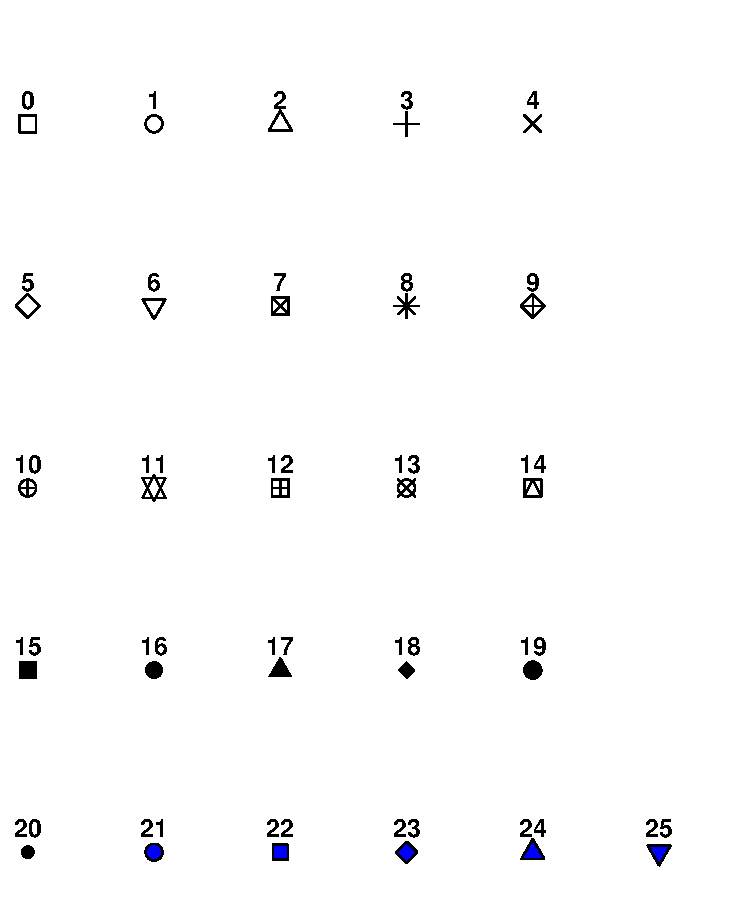
\includegraphics{Chap2_R_files/figure-beamer/unnamed-chunk-5-1} \end{center}
\end{frame}

\begin{frame}[fragile]{Les types des traits}
\protect\hypertarget{les-types-des-traits}{}
Le type de traits peut être spécifier en utilisant le paramètre
graphique \texttt{lty}. Les types de traits disponibles dans R sont :

\begin{center}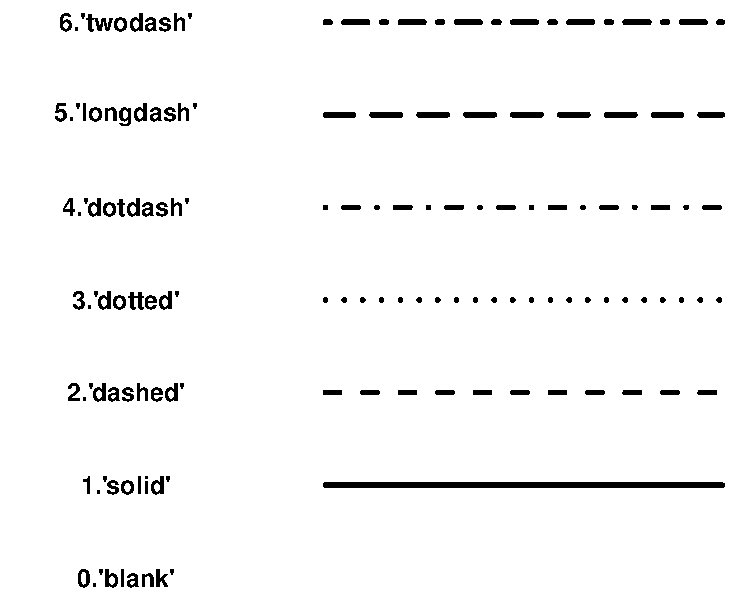
\includegraphics{Chap2_R_files/figure-beamer/unnamed-chunk-6-1} \end{center}
\end{frame}

\begin{frame}[fragile]{Ajouter un texte}
\protect\hypertarget{ajouter-un-texte}{}
Pour ajouter du texte à un graphique avec le logiciel statistique R, les
fonctions \texttt{text()} et \texttt{mtext()} peuvent être utilisées.

\begin{Shaded}
\begin{Highlighting}[]
\FunctionTok{text}\NormalTok{(x,y,label)}
\end{Highlighting}
\end{Shaded}

x et y sont les coordonnées du texte à ajouter et label est le texte à
écrire sur le graphique.

\begin{Shaded}
\begin{Highlighting}[]
\NormalTok{x1}\OtherTok{=}\FunctionTok{cos}\NormalTok{(}\FunctionTok{seq}\NormalTok{(}\DecValTok{0}\NormalTok{,pi,}\AttributeTok{len=}\DecValTok{60}\NormalTok{)); }\FunctionTok{plot}\NormalTok{(x1,}\AttributeTok{type=}\StringTok{"n"}\NormalTok{, }\AttributeTok{xlab=}\StringTok{""}\NormalTok{, }\AttributeTok{ylab=}\StringTok{""}\NormalTok{)}
\FunctionTok{text}\NormalTok{(}\DecValTok{12}\NormalTok{, x1[}\DecValTok{12}\NormalTok{], }\StringTok{"Bonjour"}\NormalTok{, }\AttributeTok{col=}\DecValTok{2}\NormalTok{); }\FunctionTok{text}\NormalTok{(}\DecValTok{40}\NormalTok{, x1[}\DecValTok{40}\NormalTok{], }\StringTok{"Hello"}\NormalTok{, }\AttributeTok{col=}\DecValTok{4}\NormalTok{)}
\FunctionTok{text}\NormalTok{(}\DecValTok{50}\NormalTok{,}\FloatTok{0.5}\NormalTok{, }\FunctionTok{expression}\NormalTok{(}\FunctionTok{hat}\NormalTok{(beta)))}
\end{Highlighting}
\end{Shaded}

\begin{center}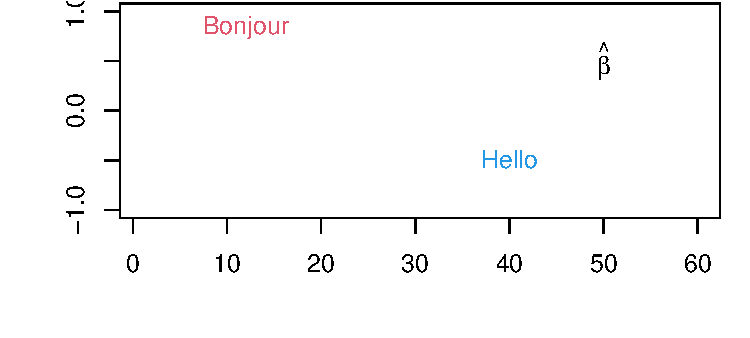
\includegraphics{Chap2_R_files/figure-beamer/unnamed-chunk-8-1} \end{center}
\end{frame}

\begin{frame}[fragile]{ggplot}
\protect\hypertarget{ggplot}{}
Une autre manière pour faire la représentation graphique est
l'utilisation de la fonction \texttt{ggplot} du package \texttt{ggplot2}
qui doit être installer par la commande
\texttt{install.package("ggplot2")}. Après l'installation, on fait appel
au package à l'aide \texttt{library("ggplot2")}.

\begin{Shaded}
\begin{Highlighting}[]
\FunctionTok{install.packages}\NormalTok{(}\StringTok{"ggplot2"}\NormalTok{)}
\FunctionTok{library}\NormalTok{(}\StringTok{"ggplot2"}\NormalTok{)}
\end{Highlighting}
\end{Shaded}

\pause

La fonction \texttt{ggplot} prend comme un premier argument une
\texttt{data.frame} qui contient les données à représenter. Un deuxième
argument \texttt{aes(x,y)} spécifie les valeurs des abscisses et les
ordonnées.
\end{frame}

\begin{frame}[fragile]
\begin{Shaded}
\begin{Highlighting}[]
\NormalTok{x}\OtherTok{=}\FunctionTok{seq}\NormalTok{(}\SpecialCharTok{{-}}\NormalTok{pi, pi, }\AttributeTok{len=}\DecValTok{100}\NormalTok{)}
\NormalTok{y}\OtherTok{=}\FunctionTok{sin}\NormalTok{(x); dd}\OtherTok{=}\FunctionTok{data.frame}\NormalTok{(x,y)}
\NormalTok{p}\OtherTok{=}\FunctionTok{ggplot}\NormalTok{(dd,}\FunctionTok{aes}\NormalTok{(x,y))}\SpecialCharTok{+}\FunctionTok{geom\_line}\NormalTok{()}
\NormalTok{p}
\end{Highlighting}
\end{Shaded}

\begin{center}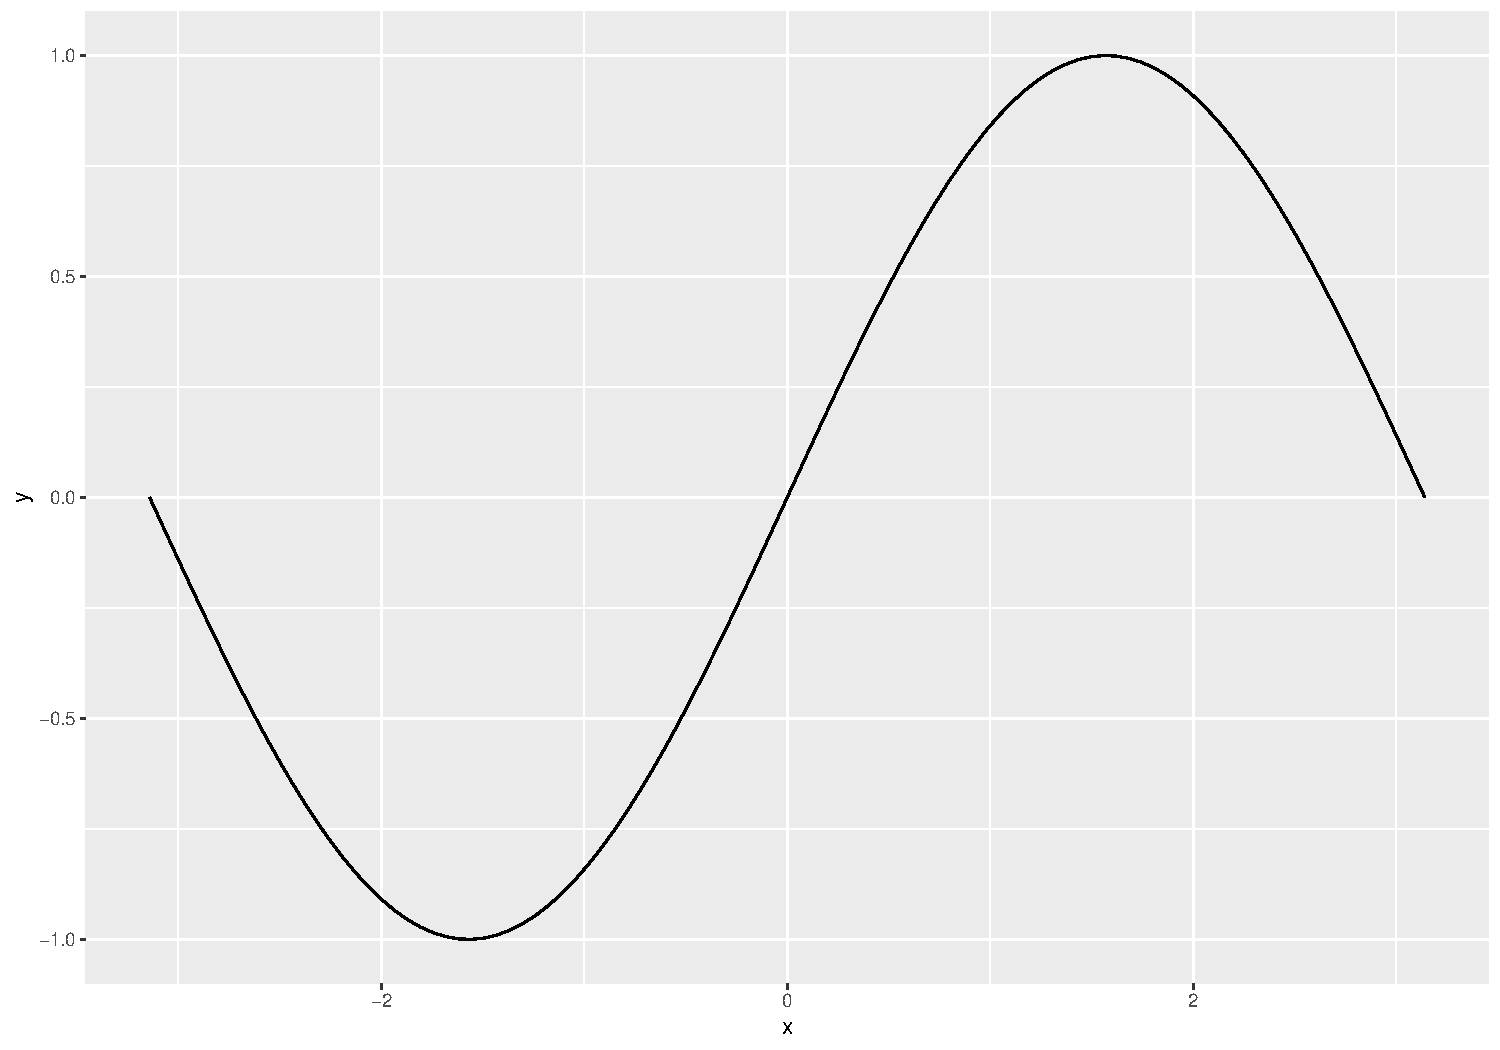
\includegraphics[height=0.7\textheight]{Chap2_R_files/figure-beamer/unnamed-chunk-10-1} \end{center}
\end{frame}

\begin{frame}[fragile]
Les paramètres de la largeur et la couleur de la courbe doivent être
spécifiés dans \texttt{geom\_line()}. L'ajout d'un titre se fait par
l'ajout de \texttt{ggtitle()}.

\begin{Shaded}
\begin{Highlighting}[]
\NormalTok{p}\OtherTok{=}\NormalTok{p}\SpecialCharTok{+}\FunctionTok{geom\_line}\NormalTok{(}\AttributeTok{linewidth=}\FloatTok{1.2}\NormalTok{, }\AttributeTok{colour=}\StringTok{"blue"}\NormalTok{)}\SpecialCharTok{+} \FunctionTok{ggtitle}\NormalTok{(}\StringTok{"Titre"}\NormalTok{)}
\NormalTok{p}
\end{Highlighting}
\end{Shaded}

\begin{center}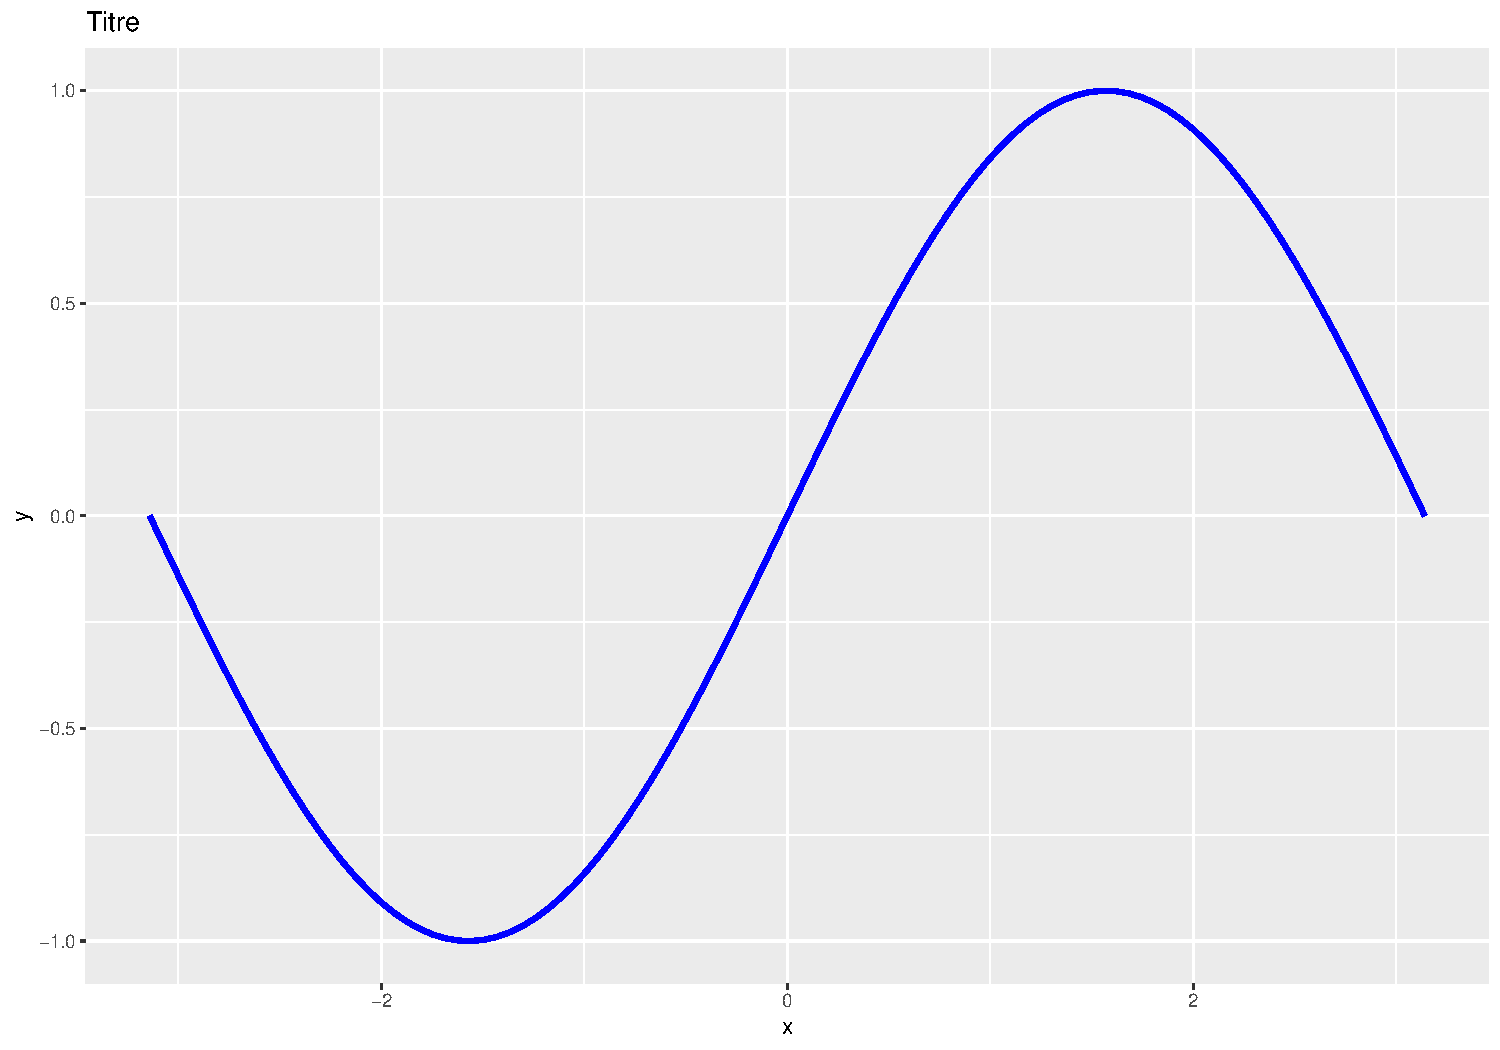
\includegraphics[height=0.7\textheight]{Chap2_R_files/figure-beamer/unnamed-chunk-11-1} \end{center}
\end{frame}

\begin{frame}[fragile]
Si on veut centrer le titre ou le mettre en couleur ou encore le mettre
en gras, on ajoutera
\texttt{theme(plot.title\ =\ element\_text(hjust\ =\ 0.5,\ size=20,\ color="darkred"))}.

\begin{Shaded}
\begin{Highlighting}[]
\NormalTok{p}\OtherTok{=}\NormalTok{p}\SpecialCharTok{+}\FunctionTok{theme}\NormalTok{(}\AttributeTok{plot.title =} \FunctionTok{element\_text}\NormalTok{(}\AttributeTok{hjust =} \FloatTok{0.5}\NormalTok{, }\AttributeTok{size=}\DecValTok{20}\NormalTok{,}
          \AttributeTok{color=}\StringTok{"darkred"}\NormalTok{))}\SpecialCharTok{+}\FunctionTok{labs}\NormalTok{(}\AttributeTok{x=}\StringTok{""}\NormalTok{,}\AttributeTok{y=}\StringTok{""}\NormalTok{)}
\NormalTok{p}
\end{Highlighting}
\end{Shaded}

\begin{center}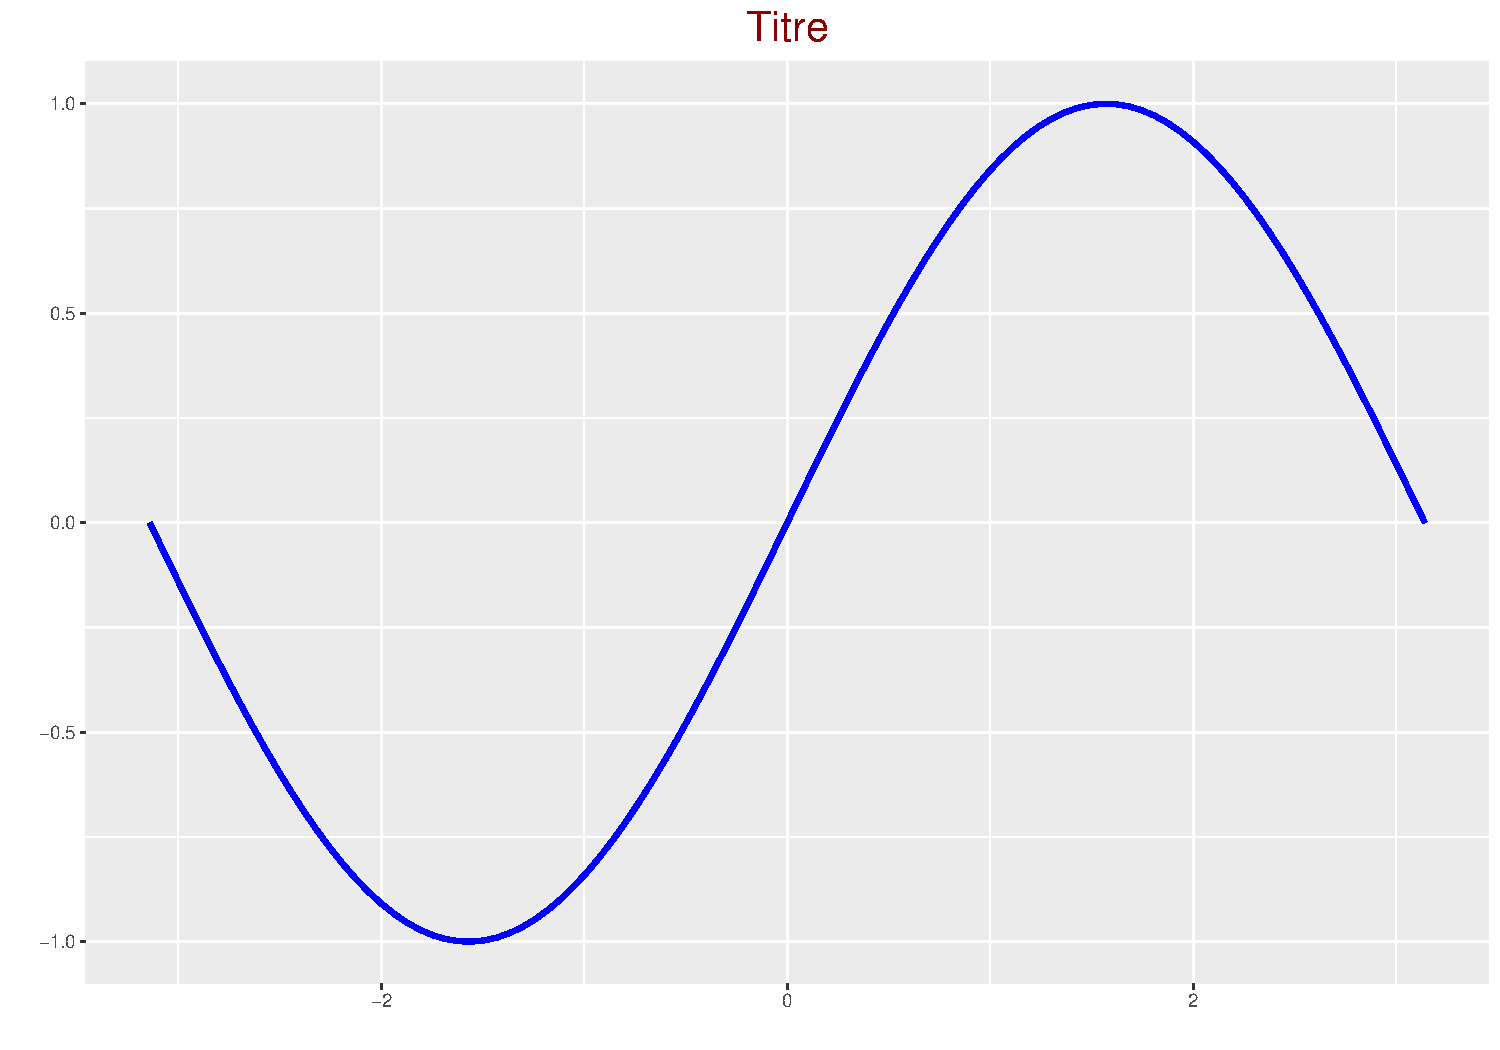
\includegraphics[height=0.67\textheight]{Chap2_R_files/figure-beamer/unnamed-chunk-12-1} \end{center}
\end{frame}

\hypertarget{statistique-univariuxe9e}{%
\section{Statistique univariée}\label{statistique-univariuxe9e}}

\begin{frame}{Statistique univariée}
On entend par \(\color{red}{\textbf{statistique univariée}}\) l'étude
d'une seule variable, que celle-ci soit
\(\color{blue}{\textbf{qualitative}}\) ou
\(\color{blue}{\textbf{quantitative}}\). La statistique univariée fait
partie de la statistique descriptive.

\pause

Une \textbf{variable qualitative} (aussi appelée variable catégorique)
réfère à une caractéristique qui n'est pas quantifiable. Une variable
catégorique peut être nominale ou ordinale. \pause

\begin{itemize}
\item
  Une variable \(\color{violet}{\textbf{nominale}}\) décrit un nom, une
  étiquette ou une catégorie sans ordre naturel. Le sexe est un exemple.
\item
  Une variable \(\color{violet}{\textbf{ordinale}}\) est une variable
  dont les valeurs sont définies par une relation d'ordre entre les
  catégories possibles. La variable mention est une variable ordinale
  parce que la catégorie ``très bien'' est meilleure que la catégorie
  ``bien'' qui est meilleure de la catégorie ``passable''.\pause
\end{itemize}

Une \textbf{variable quantative} est une caractéristique quantifiable
dont les valeurs sont des nombres. Les variables numériques peuvent être
\(\color{blue}{\textbf{continues}}\) ou
\(\color{blue}{\textbf{discrètes}}\).\pause

\begin{itemize}
\item
  Variables continues: On dit qu'une variable est
  \(\color{violet}{\textbf{continue}}\) si elle prend un nombre infini
  de valeurs réelles possibles à l'intérieur d'un intervalle donné.
  Prenons la taille d'un élève par exemple.\pause
\item
  Variables discrètes: Contrairement à une variable continue, une
  variable \(\color{violet}{\textbf{discrète}}\) ne peut prendre qu'un
  nombre fini de valeurs réelles possibles à l'intérieur d'un intervalle
  donné. Le nombre d'enfants dans un ménage est un exemple.
\end{itemize}
\end{frame}

\hypertarget{variable-qualitative}{%
\section{Variable qualitative}\label{variable-qualitative}}

\begin{frame}{Variable qualitative}
Une variable qualitative peut être représentée, soit par un diagramme à
barres, soit par un diagramme en secteurs.\pause

\(\color{red}{\textbf{Exemple:}}\)

En 2005, les recettes du budget de l'Etat se présentaient de la façon
suivante (en milliards) :

\begin{longtable}[]{@{}lllllll@{}}
\toprule
\endhead
Source & TVA & IR & IS & TPP & AI & RNF \\
RF & 348 & 163 & 71 & 54 & 161 & 41 \\
\bottomrule
\end{longtable}

\vspace*{4cm}
\end{frame}

\end{document}
